\section{Optimum transfer}

Once direct transfers (prograde and retrograde) have been computed for each pair
of launch and arrival dates, the most optimum transfer orbit can be identified.

It is important to define the concept of optimum transfer. In this context, this
term refers to the orbit whose launch energy is the lowest. Other mission
constrains may be considered but for the purpose of this work, the launch $C_3$
energy is the only parameter considered. The reason is that the $\Delta v_1$
required for a direct transfer is a limiting factor for nowadays technology.

Porkchps represented in figures \ref{fig:oumuamua-direct-prograde-transfer-porkchop} and
\ref{fig:borisov-direct-prograde-transfer-porkchop}


contain an optimum transfer maneuver. This is the maneuver
for which the $C_3$ energy is minimized. Table \ref{tab:direct-transfer-optimum}
collects the values for the launch and arrival dates, and the
characteristic energy for the most optimum transfer.

\subsection{'Oumuamua}

Among the prograde and retrogade direct transfers, the most optimum transfer is
contained in the set of prograde orbits. Analyzing figure
\ref{fig:oumuamua-direct-prograde-transfer-porkchop} reveals that the lowest
characteristic energy is the one collected in table \ref{tab:oumua-direct-transfer-optimum}.

\vspace{0.5cm}
\begin{table}[H]
  \centering
  \begin{tabular}{|c|c|c|c|}
    \hline
    Object & Launch date & Arrival date & Required $C_3$ [km$^2$/s$^2$] \\
    \hline
    1I/'Oumuamua & 2017-08-15 & 2032-05-13 & 720.28 \\
    \hline
  \end{tabular}
  \caption{Optimum transfer orbit for a direct transfer between the Earth and 1I/'Oumuamua.}
  \label{tab:oumua-direct-transfer-optimum}
\end{table}

\begin{figure}[H]
  \centering
  \includegraphics[width=0.9\textwidth]{static/oumuamua/direct-optimum-transfer.png}
  \caption{Optimum direct transfer orbit between Earth and 1I/'Oumuamua. The
    high speed of 'Oumuamua one passing through its perihelion leads to a low
    resolution in the sampling of points close to this region.}
  \label{fig:oumuamua-direct-transfer-orbit}
\end{figure}

Figure \ref{fig:oumuamua-direct-transfer-orbit} shows the trajectory of the
optimum transfer between Earth and 1I/'Oumuamua. Impulses for this maneuver are
described in table \ref{tab:oumuamua-direct-transfer-impulses}. Total cost is
$42.00$ km/s.

\begin{table}[H]
  \centering
  \begin{tabular}{|c|c|c|c|}
    \hline
    Impulse & $\Delta v_x$ [km/s] & $\Delta v_y$ [km/s] & $\Delta v_z$ [km/s] \\
    \hline
    Launch & 28.20 & -30.10 & 3.91 \\
    \hline
    Arrival & 0.28 & -0.49 & -0.02 \\
    \hline
  \end{tabular}
  \caption{Impulses required for the optimum transfer between Earth and 1I/'Oumuamua.}
  \label{tab:oumuamua-direct-transfer-impulses}
\end{table}

This scenario was analyzed by \cite{hein2018} too. However, the analysis
presented in this work expands previous article by covering the retrograde case
and providing the optimum solution.

Despite having found and optimum solution, the value of $C_3 = 720.28$
km$^2$/s$^2$ is still a high value for orbit transfers.

\subsection{Borisov}

Regarding Borisov, the most optimum transfer is also a prograde transfer. The
analysis of figure \ref{fig:borisov-direct-prograde-transfer-porkchop} shows
that the lowest characteristic energy is the one collected in table
\ref{tab:borisov-direct-transfer-optimum}.

Previously found literature shows that \cite{hibberd2021} analyzed the direct
transfer to the interloper, where he states that the optimum transfer happens 

Impulses for this maneuver are described in table
\ref{tab:borisov-direct-transfer-impulses}. Total cost is $36.95$ km/s.

\begin{table}[H]
  \centering
  \begin{tabular}{|c|c|c|c|}
    \hline
    Impulse & $\Delta v_x$ [km/s] & $\Delta v_y$ [km/s] & $\Delta v_z$ [km/s] \\
    \hline
    Launch & -11.92 & 3.69 & -25.73 \\
    \hline
    Arrival & 0.58 & -5.37 & -6.37 \\
    \hline
  \end{tabular}
  \caption{Impulses required for the optimum transfer between Earth and 2I/Borisov.}
  \label{tab:borisov-direct-transfer-impulses}
\end{table}


\vspace{1cm}
\begin{table}[H]
  \centering
  \begin{tabular}{|c|c|c|c|}
    \hline
    Object & Launch date & Arrival date & Required $C_3$ [km$^2$/s$^2$] \\
    \hline
    2I/Borisov & 2016-04-28 & 2032-01-15 & 820.06 \\
    \hline
  \end{tabular}
  \caption{Optimum transfer orbit for a direct transfer between the Earth and 2I/Borisov.}
  \label{tab:borisov-direct-transfer-optimum}
\end{table}

Figure \ref{fig:borisov-direct-transfer-orbit} shows the trajectory of the
optimum transfer between Earth and 2I/Borisov.

\begin{figure}[H]
  \centering
  \includegraphics[width=\textwidth]{static/borisov/direct-optimum-transfer.png}
  \caption{Optimum direct transfer orbit between Earth and 2I/Borisov. This
        trajectory does not pass close to the Sun. However, the transfer requires almost $820$
        km$^2$/s$^2$ to achieve a targeting with the interloper.}
  \label{fig:borisov-direct-transfer-orbit}
\end{figure}
